\documentclass[12pt,twoside,a5paper]{amsbook}

\usepackage[usenames,dvipsnames]{color}
\usepackage{epsfig,exscale}
\usepackage[latin1]{inputenc}
\usepackage{hyperref}
 
\usepackage{setspace}
\onehalfspacing

\usepackage[includeheadfoot,
top=20mm,
left=30mm=,
right=20mm,
bottom=15mm
]{geometry}

\renewcommand{\chaptername}{}
\renewcommand{\thechapter}{\Roman{chapter}}
\renewcommand{\contentsname}{�ndice}
\newcommand{\dlg}{\noindent $\bullet$ }

\hypersetup{
pdftitle={Cuentos para ir a dormir},
pdfsubject={cuentos},
pdfauthor={Ariel Narv�ez},
pdfkeywords={cuentos}
}

\title[Cuentos]{CUENTOS PARA IR A DORMIR} 
\author[Ariel Narv�ez]{Ariel Narv�ez}


\begin{document}
\maketitle

\tableofcontents

\chapter{EL COCODRILO Y LAS HORMIGAS}
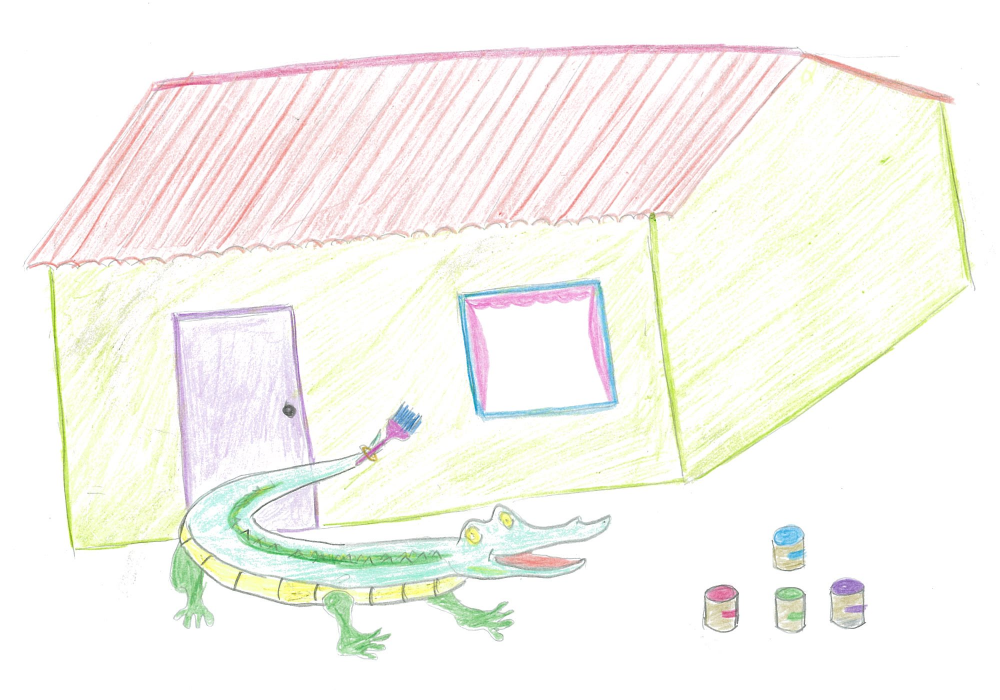
\includegraphics[width=0.8\textwidth]{pics/cocodrilo_1.png}

Un d�a de verano, el cocodrilo como hace varios d�as ten�a ya
preparado, se levant� muy temprano y tras un muy buen desayuno se
dispuso a pintar su casa. Su casa no era muy grande pero ten�a un gran
jard�n con muchas plantas. El cocodrilo ten�a preparado muchas brochas
y todos los colores para las distintas partes de la casa: El techo lo
iba a pintar rojo; las ventanas, azules; la puerta, lila; las paredes,
verdes y la cerca que rodea al jard�n, blanca.

El cocodrilo estuvo pintando sin descanzo durante toda la
ma�ana. Aparte de tomar la brocha sus manos tambi�n utiliz� su cola
para poder as� pintar los rincones dif�ciles de alcanzar. Un poco
antes del medio d�a, el cocodrilo termin� de pintar toda su
casa. Aunque ya ten�a mucha hambre, antes de empezar a cocinar su
almuerzo orden� todos los materiales que utiliz� para pintar. 

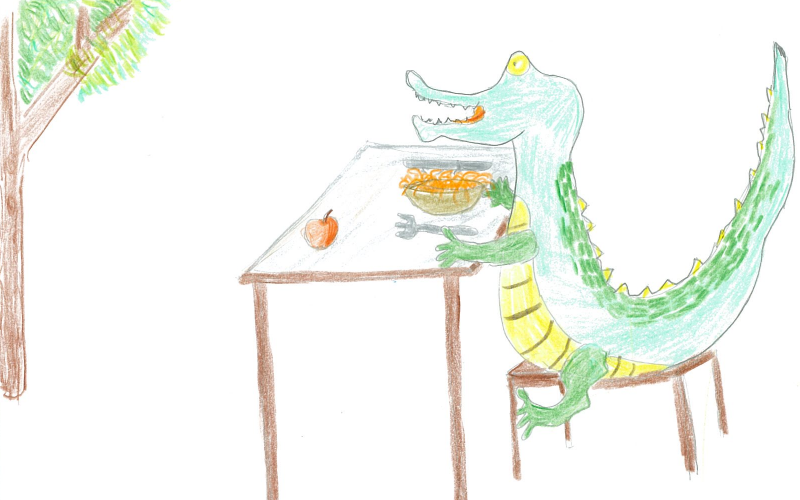
\includegraphics[width=0.8\textwidth]{pics/cocodrilo_2.png}

Su almuerzo consisti� en unos ricos tallarines con salsa y para el
postre ten�a preparada una manzana, pero decidi� ir a descanzar a la
orilla del r�o para luego comer la manzana. En la orilla del rio el
cocodrilo ten�a una mesa y una silla en la cual disfrutaba de tomar
sol en el verano antes de meterse a nadar al r�o. Esta vez no fue la
excepci�n y dej� la manzana sobre la mesa y disfruto del sol en la
silla. Luego de una reponedora siesta, el cocodrilo se meti� al
r�o a nadar. Aunque el r�o ten�a un fuerte caudal, el cocodrilo no
ten�a problemas para nadar con la ayuda de su fuerte cola y con
facilidad cruzaba el r�o de un lado a otro.

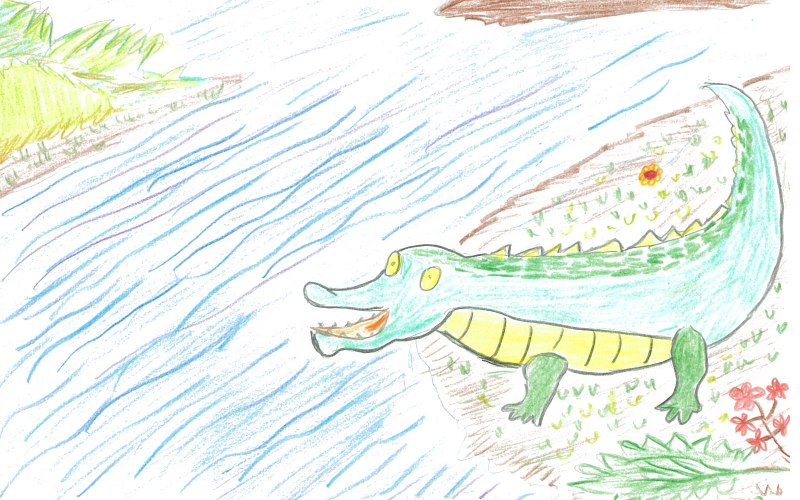
\includegraphics[width=0.8\textwidth]{pics/cocodrilo_3.png}

Al termininar de nadar y disponerse a comer la manzana, el cocodrilo
se encontr� con una sorpresa: la manzana ya no se encontraba sobre la
mesa. El cocodrilo empez� a buscar la manzana, y r�pidamente la
encontr� bajo la mesa, pero algo raro ocurr�a, la manzana lentamente
se mov�a. Al acercarse y mirar detenidamente, el cocodrilo se dio
cuenta que unas hormigas se llevaban su manzana. El cocodrilo les dijo
que le devolvieran su manzana a lo que las hormigas le
res\-pon\-die\-ron: 

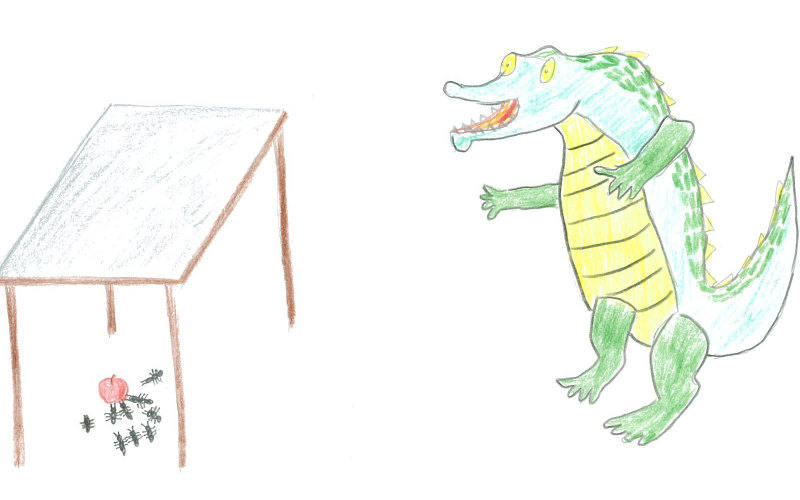
\includegraphics[width=0.8\textwidth]{pics/cocodrilo_4.png}

\dlg  Nosotras somos muchas y tenemos hambre!!! \\
\dlg El cocodrilo muy enojado les dijo: \\
\dlg  si tienen tanta hambre vayan ustedes mismas a buscar
manzanas al �rbol y no me quiten la m�a. \\
\dlg Las hormigas respondieron muy sorprendidas:\\
\dlg  Cu�l �rbol? \\
\dlg Las hormigas no conoc�an el �rbol as� que muy curiosas le
preguntaron al cocodrilo: \\
\dlg  D�nde est� el manzano? \\
\dlg El cocodrilo aunque estaba muy enojado les respondi�
amablemente y les dijo que simplemente ellas ten�an seguir el r�o y
caminar unos 10 minutos y se encontrar�an con el manzano.

Las hormigas le devolvieron la manzana al cocodrilo y partieron
r�pidamente a buscar manzanas. Cuando llegaron al �rbol todas las
hormigas se subieron y sacaron una manzana para cada una.  Adem�s
buscaron la manzana m�s roja y grande del �rbol y se la llevaron de
regalo al cocodrilo para agrecerle por ense�arles la ubicaci�n del
manzano y para pedirle perd�n por tratar de llevarse su manzana.

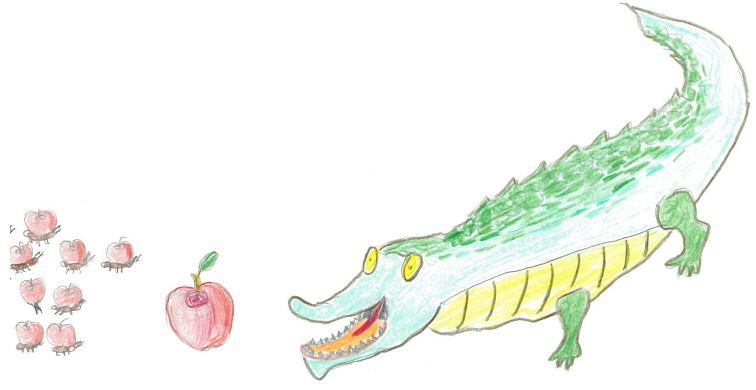
\includegraphics[width=0.8\textwidth]{pics/cocodrilo_5.png}


\chapter{EL LIBRO BENJAMIN}
%%\includegraphics[width=0.6\textwidth]{pics/benjamin} 



\chapter{LAS HORMIGAS Y EL TOPO}
Durante todo el verano las Hormigas se fueron a la playa. 
%
Algunas se dedicaron a jugar voleibol, otras al f�tbol, otras a las
paletas, otras a nadar, otras constru�an castillos de arena y las
restantes simplemente disfrutaban del sol.

Cuando el verano acababa, la jefa de las Hormigas llam� a una
reuni�n. La jefa con voz de mando dijo: \\
\dlg Hermanas, nuestras vacaciones en la playa se terminan
hoy. 
%
\fgr{hormigas_1.png}
%
A partir de ma�ana comenzamos la recolecci�n de alimentos para el
duro invierno que viene. 
%
Tenemos dos meses para la recolecci�n y despu�s debemos construir un
hogar para nosotras y nuestra comida.

Todas las Hormigas escuchaban muy atentamente. 
%
La Hormiga secretaria tomaba nota de todo lo que dec�a la jefa.
%
�sta segu�a con su plan: \\
\dlg  Los alimentos necesarios son: trigo, ma�z, arroz, manzanas,
peras, papas, leche, miel, porotos, lentejas y arvejas. 
%
%\fgr{hormigas_2.png}
%
Para eso nos dividiremos en escuadras que se dedicar�n a recolectar
cada uno de estos alimentos. 
%
Mi secretaria ac� tiene la lista con las escuadras.

Para terminar la jefa le dijo al resto de las Hormigas: \\
\dlg Ma�ana comenzamos muy temprano as� que hoy disfruten lo m�s
posible de la playa por que ser� el �ltimo y luego se nos viene un
duro trabajo.

Al d�a siguiente y durante las siguientes semanas las Hormigas
trabajaron sin cesar. 
%
Luego de dos meses de recolecci�n, las Hormigas ya ten�an suficiente
alimentos para el invierno y deb�an ahora iniciar la construcci�n de
su hogar. 
%
Por alguna extra�a raz�n, ese a�o el invierno se adelant� y las
Hormigas a�n no ten�an listo su hogar cuando la nieve ya hab�a
llegado. 
%
Esto era un problema muy grave. 
%
La jefa de las Hormigas les dijo a sus compa�eras: \\
\dlg Debemos encontrar pronto un hogar para nosotras y 
nuestra comida... \\
\noindent En ese momento el Papagayo que miraba desde arriba 
interrumpi� a la jefa y le dijo: \\
\dlg Seg�n lo que yo s�, el Topo agrand� su casa durante el 
verano y tiene, por tal, unas piezas libres que les podr�an 
ser �tiles. 
%
\fgr{hormigas_3.png}
%
Yo ir� r�pidamente a preguntarle.
%
El Papagayo sali� volando r�pidamente y se encontr� con el Topo
explic�ndole el problema de las Hormigas. 
% 
El Topo respondi� r�pida y amablemente: \\
\dlg Ning�n problema, que vengan a vivir conmigo durante el invierno.\\
%
El Papagayo vol� de vuelta y le dio la buena noticia a la Hormigas. 
%
La jefa de la Hormigas r�pidamente organiz� el viaje hasta la casa del
Topo. 
%
Al llegar a la casa del Topo las Hormigas saludaron y agradecieron su
amabilidad.
%
El Topo les respondi�: \\
\dlg Gracias a ustedes que me van a acompa�ar durante el invierno. 
%
Yo vivo solo, trabajo durante todo el d�a afuera y llego muy cansado
en la tarde. 
%
\fgr{hormigas_4.png}

Ese invierno fue muy entretenido para las Hormigas y el Topo. 
%
Las Hormigas usando toda la comida que hab�an recolectado le cocinaban
al Topo una rica cena para cuando �ste llegaba cansado de su trabajo y
despu�s antes de dormir jugaban a las cartas o miraban alguna pel�cula
juntos.





\chapter{EL MENSAJE}

\chapter{EL TOPO Y EL MONO}

\chapter{LA MANZANA}
Un d�a iban caminando juntos por el campo tres animales muy grandes:
un Elefante, una Girafa y un Dinosaurio. Iban de lo mas felices
conversando cuando se dieron cuenta que en frente de ellos
hab�a un manzano con la �ltima de sus manzanas en el tope de su frondosa
copa.

El primero en decir que la manzana le pertenec�a fue el Elefante, que
dijo de inmediato:\\
\dlg  Esa manzana es m�a, la voy a sacar y me la voy a comer. \\
La Girafa y el Dinosaurio al un�sono replicaron la misma respuesta: \\
\dlg  Yo tambi�n la puedo sacar y me la como.

En resumen, los tres querian la manzana y cada uno estaba muy seguro
que debido a su tama�o no ser�a un problema poder sacala aunque la
manzana en realidad se ubicaba a mucha latura. Luego de discutir el
tema llegaron a un acuerdo: Ser�a la Jirafa la primera en intentar
sacar la manzana, luego vendr�a el Elefante y por �ltimo el Dinosaurio
que era el m�s grande de los tres y de seguro sacar�a la manzana.

La Jirafa se acerc� al �rboly con estir� su largo cuello para poder
alcanzar la manzana. Aun con su mejor esfuerzo, tratando incluso de
pararse s�lo en sus patas traseras, la Jirafa no fue capaz de alcanzar
la manzana. Al darse por vencida, le dio el turno al Elefante. �ste se
acerc� se par� en sus patas traseras y estir� su larga y fuerte trompa
pero no alcanzaba la manzana. Incluso con su trompa intent� zamarrear
las ramas para poder as� botar la manzana. Esto tampoco result�.

Finalmente se acerc� al manzano el Dinosaurio muy seguro de sacar la
manzana, estir� su largo cuello y lo dirigi� haci� la manzana pero
para su sorpresa no la pudo alcanzar. Luego de intentarlo varias veces
se convenci� de que le era imposible.

Los tres m�s grandes animales se encontraban completamente
sorprendidos de que ninguno de ellos fue capaz de sacar la manzana. 

En ese momento se acerca al manzano un peque�o mono que empieza a
escalar y saltar de rama en rama subiendo r�pidamente a la copa del
�rbol. Con la mirada at�nita del Elefante, la Jirafa y el Dinosaurio;
el peque�o mono fue capaz de sacar la manzana y muy feliz bajar del
�rbol comi�ndosela. Los saludo afectuosamente y tan repent�namente
como lleg�, se fue. 

El Elefante, la Jirafa y el Dinasaurio al un�sono se rieron de lo que
hab�a pasado y siguieron su camino.


\end{document}

